\documentclass[12pt,a4paper]{article}
\usepackage{vntex} % Tiếng Việt
\usepackage{graphicx} % Chèn hình ảnh
\usepackage{listings} % Thêm gói listings để chèn code
\usepackage{xcolor} % Màu cho code
\usepackage{changepage} % Thay đổi lề
\lstset{
    language=R,
    basicstyle=\footnotesize\ttfamily,
    numbers=none,
    numberstyle=\tiny\color{gray},
    stepnumber=1,
    numbersep=0.01pt,
    tabsize=2,
    breaklines=true,
    breakatwhitespace=false,
    xleftmargin=0cm, % for line numbers
    framexleftmargin=0cm, % for code frame
    keywordstyle=\color{blue},
    commentstyle=\color{green},
    stringstyle=\color{orange},
    frame=single,
    rulecolor=\color{black},
    basicstyle=\ttfamily,
}
% Thiết lập bảng
\usepackage{diagbox}
\usepackage{array}
\usepackage{tabularx}
\usepackage{longtable} % Tạo bảng qua nhiều trang
\usepackage{cellspace}
\usepackage{bm} % Chữ in đậm trong công thức toán 
\usepackage{a4wide,amssymb,epsfig,latexsym,multicol,array,hhline,fancyhdr}
\usepackage{tikz}
\usepackage{color}
\usepackage{subcaption}
\usepackage{framed}
\usepackage{float} % Để chèn hình ảnh vào đúng vị trí
\usepackage{fancyvrb} %Đưa dữ liệu dạng nguyên thủy vào
\usepackage{amsmath} % Công thức toán
\usepackage{slashbox} % Chèn đường chéo trong bảng
% Thiết lập kích thước
\usepackage{geometry}
\geometry{
    left=3cm,
    right=2cm,
    top=2.5cm,
    bottom=2.5cm,
}
\usepackage{hyperref} %Chèn link
\hypersetup{urlcolor=black,linkcolor=black,citecolor=black,colorlinks=true} % Màu cho các đường nét
\everymath{\color{black}}
\setlength{\headheight}{40pt}
\pagestyle{fancy}


%Header
\fancyhead{} % clear all header fields
\fancyhead[L]{
 \begin{tabular}{rl}
    \begin{picture}(25,15)(0,0)
    \put(0,-8){
\includegraphics[width=12mm, height=12mm]{pictures/hcmut.png}}
    %\put(0,-8){\epsfig{width=10mm,figure=hcmut.eps}}
   \end{picture}&
	%
\includegraphics[width=8mm, height=8mm]{hcmut.png} & %
	\begin{tabular}{l}
		\textbf{\bf \ttfamily Trường Đại Học Bách Khoa - ĐHQG TP.Hồ Chí Minh}\\
		\textbf{\bf \ttfamily Khoa Cơ Khí - Bộ môn Cơ Điện Tử}
	\end{tabular} 	
 \end{tabular}
}
\fancyhead[R]{
	{\tiny \bf \quad} % Khoảng trắng nhỏ trong header bên phải
}

%Footer
\fancyfoot{} % clear all footer fields
\fancyfoot[L]{\scriptsize \ttfamily Trang bị điện - điện tử trong máy công nghiệp}
\fancyfoot[R]{\scriptsize \ttfamily Trang {\thepage}/11}
\renewcommand{\headrulewidth}{0.3pt}
\renewcommand{\footrulewidth}{0.3pt}

\begin{document}
    \begin{titlepage}   
    \begin{center}
        \vspace*{-2cm} 
        \large
        \textbf{ĐẠI HỌC QUỐC GIA THÀNH PHỐ HỒ CHÍ MINH \\
        TRƯỜNG ĐẠI HỌC BÁCH KHOA\\
        KHOA CƠ KHÍ\\
        BỘ MÔN CƠ ĐIỆN TỬ}\\
        
\includegraphics[width=70mm, height=70mm]{pictures/hcmut.png} \\
        \rule{\linewidth}{0.5mm}\\
        \vspace{0.8cm}
        \Large
        \textbf{TRANG BỊ ĐIỆN - ĐIỆN TỬ TRONG MÁY CÔNG NGHIỆP}\\
        \vspace*{0.5cm}
        \Huge
        \textbf{EXERCISE 4}\\
        \vspace{0.5cm}
        \rule{\linewidth}{0.5mm}\\
        \vspace{0.8cm}
        \vspace{1cm}
        \large
        GVHD: TS. LÊ ĐỨC HẠNH\\
        \vspace{0.5cm}
        DANH SÁCH THÀNH VIÊN:\\[0.3cm]
        \begin{tabular}{|>{\centering\arraybackslash}m{1cm}|>{\centering\arraybackslash}m{7cm}|>{\centering\arraybackslash}m{5cm}|}
            \hline
            \textbf{STT} & \textbf{Họ và tên} & \textbf{MSSV} \\
            \hline
            1 & Võ Hữu Dư & 2210604 \\
            \hline
            2 & Dương Quang Duy & 2210497 \\
            \hline
            3 & Trần Quang Đạo & 2210647 \\
            \hline
        \end{tabular}
    \end{center}
        
    \vfill
    \large
    \begin{center}
        TP.HCM, \today
    \end{center}
\end{titlepage}

	\tableofcontents
	\newpage
	\section{Design a control circuit for described operation below:}
\subsection{Push button start.}
\subsubsection{Motor 1 (AC1phase), Motor2(3phase) run in star mode, after 5s motor 1 change direction, motor 2 change from star to delta, motor 3 start running.}
Motor 1 (AC1phase), Motor 2 (3phase) run in star mode:
\begin{figure}[H]
    \centering
    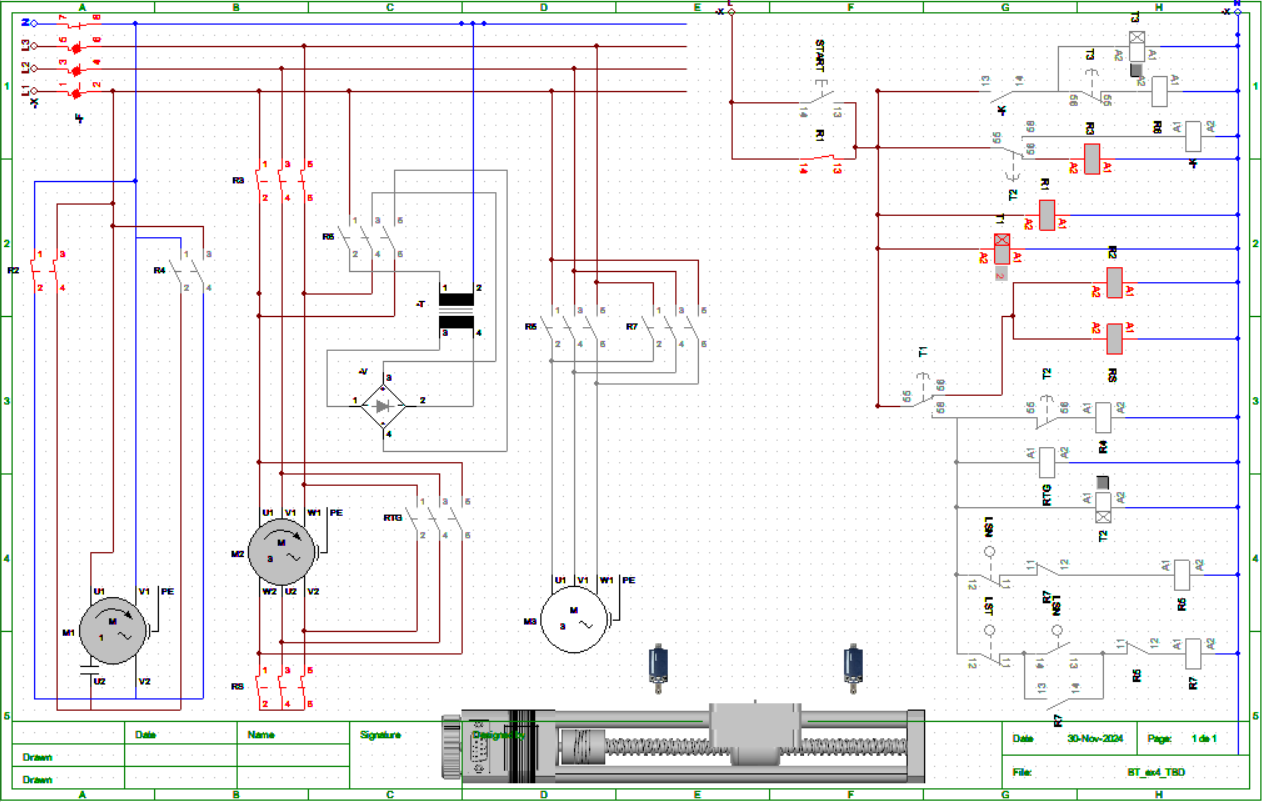
\includegraphics[width=1\textwidth]{pictures/1a.png}
\end{figure}
\cleardoublepage
After 5s motor 1 change direction, motor 2 change from star to delta, motor 3 start running:
\begin{figure}[H]
    \centering
    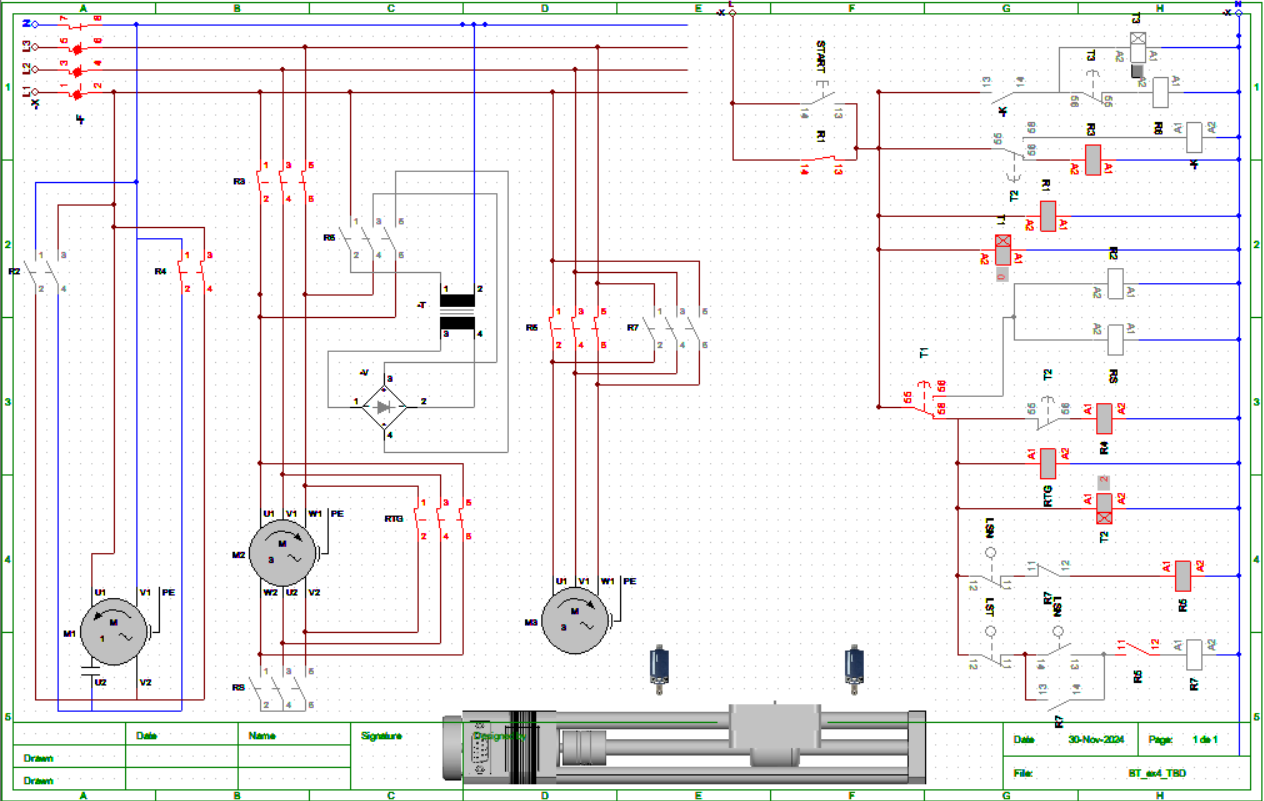
\includegraphics[width=1\textwidth]{pictures/1b.png}
\end{figure}
\cleardoublepage
\subsubsection{Motor 3 (3phase) runs from left to right then meets a limit switch then return to right then loop again,  while in 5s later motor1 stops and motor2 stop (kinematic).}
Motor 3 (3phase) runs from left to right then meets a limit switch then return to right then loop again:
\begin{figure}[H]
    \centering
    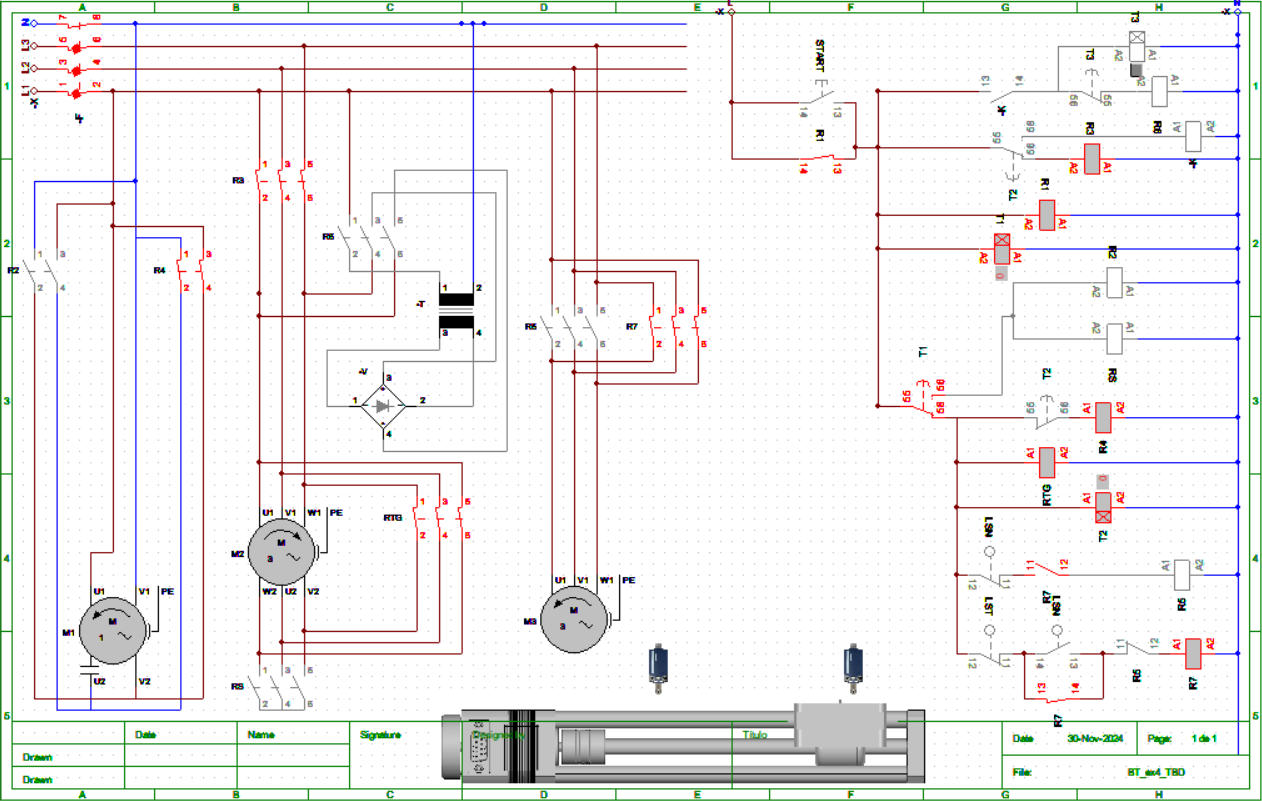
\includegraphics[width=1\textwidth]{pictures/1c.png}
\end{figure}
\cleardoublepage
In 5s later motor 1 stops and motor 2 stop (kinematic):
\begin{figure}[H]
    \centering
    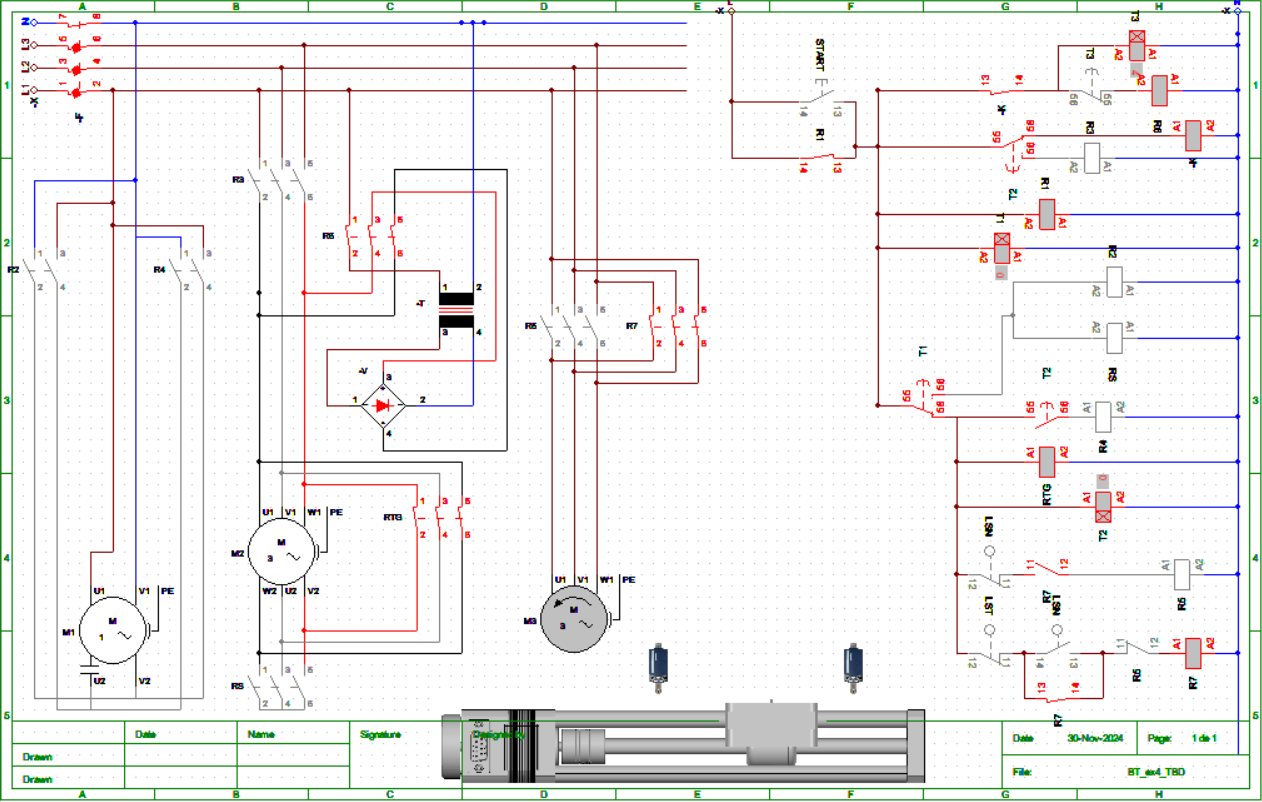
\includegraphics[width=1\textwidth]{pictures/1d.png}
\end{figure}
\cleardoublepage
\subsection{Circuit have emergency stop button.}
\subsubsection{Before the emergency stop button is pressed}
\begin{figure}[H]
    \centering
    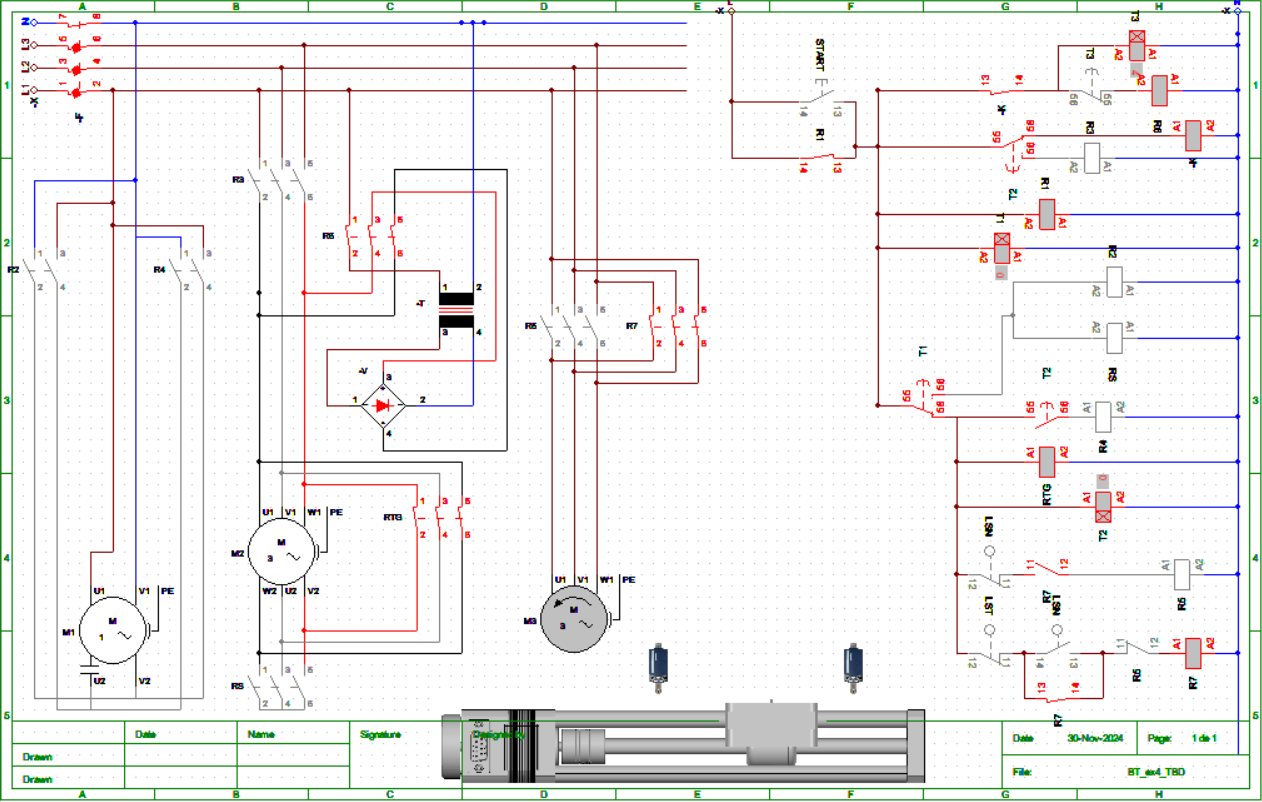
\includegraphics[width=1\textwidth]{pictures/1d.png}
\end{figure}
\cleardoublepage
\subsubsection{After the emergency stop button is pressed}
\begin{figure}[H]
    \centering
    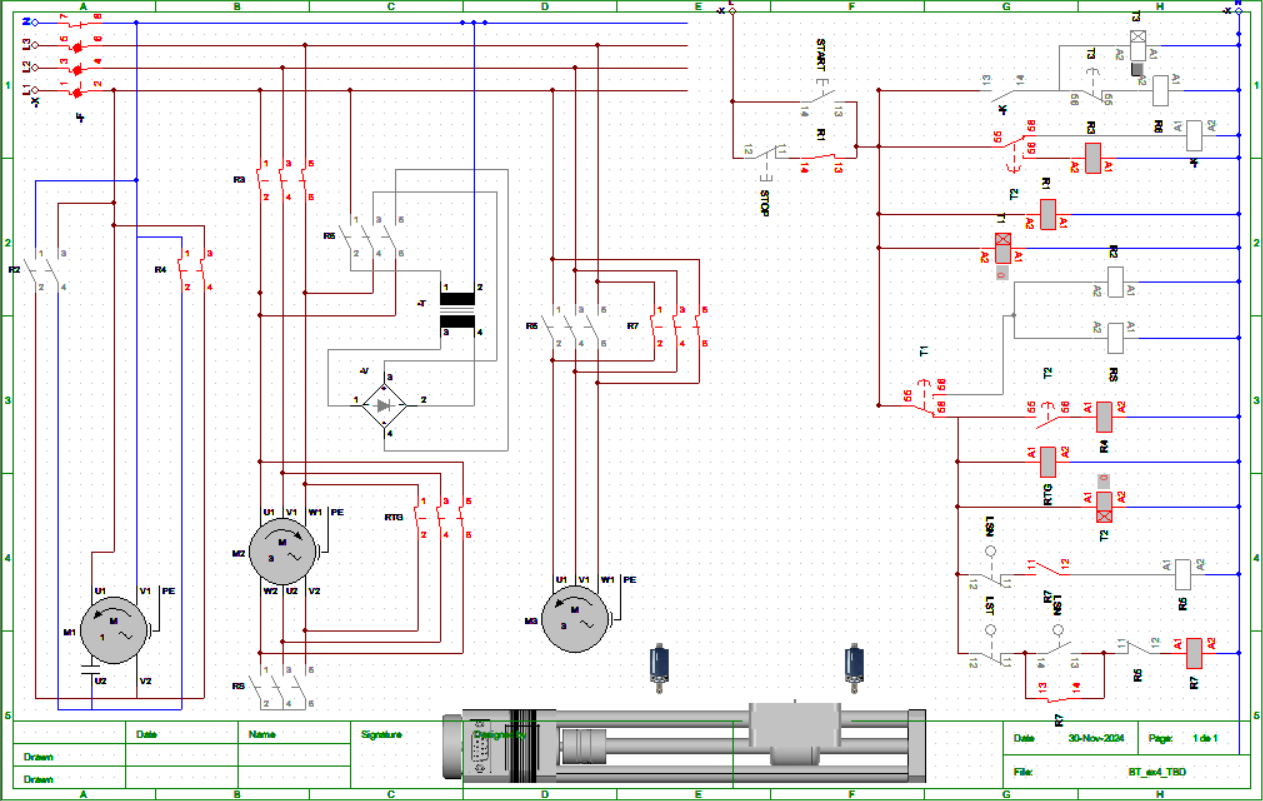
\includegraphics[width=1\textwidth]{pictures/1e.png}
\end{figure}
$\Rightarrow$ After the emergency stop button is pressed, all motors stop immediately and will not reactivate until the start button is pressed.
\cleardoublepage
\end{document}